  
\begin{minipage}{0.48\linewidth}
Un \textbf{cylindre de révolution} est le solide de l'espace obtenu en faisant tourner un rectangle autour d'un axe, appelé \og axe de révolution \fg{}. Il a:
\begin{itemize}
\item deux bases qui sont des disques de mêmes rayons et superposables.
\item l'enveloppe latérale \og dépliée \fg{} est un rectangle. 
\end{itemize}
\end{minipage} 
\hfill
\begin{minipage}{0.48\linewidth}
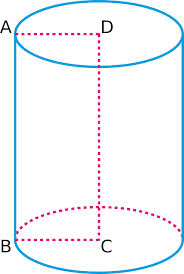
\includegraphics[scale=0.5]{RepS-cylindre.jpg} 
\end{minipage} 